\label{implementation}

This chapter explains implementation details of \tbas\ running on \thismachine.

\section{Keycodes}

\index{keycodes}This is a table of keycodes recognised by the LibGDX, a framework that \thismachine\ runs on.

\begin{longtable}{*{2}{m{\textwidth}}}\hline
\endfirsthead
\endhead

\endfoot
\hline
\endlastfoot
\centering
\begin{tabulary}{\textwidth}{rl}
Key & Code \\
\hline
\ttfamily{1} & 8 \\
\ttfamily{2} & 9 \\
\ttfamily{3} & 10 \\
\ttfamily{4} & 11 \\
\ttfamily{5} & 12 \\
\ttfamily{6} & 13 \\
\ttfamily{7} & 14 \\
\ttfamily{8} & 15 \\
\ttfamily{9} & 16 \\
\ttfamily{0} & 17 \\
$\hookleftarrow$ & 66 \\
\condensedfont{BkSp} & 67 \\
\condensedfont{Tab} & 61 \\
\ttfamily{`} & 68 \\
\ttfamily{'} & 75 \\
\ttfamily{;} & 43 \\
\ttfamily{,} & 55 \\
\ttfamily{.} & 56 \\
\ttfamily{/} & 76 \\
\ttfamily{[}\hspace*{0.083em} & 71 \\
\ttfamily{]}\hspace*{-0.083em} & 72 \\
\ttfamily{-} & 69 \\
\end{tabulary}
\begin{tabulary}{\textwidth}{rl}
Key & Code \\
\hline
\ttfamily{+} & 70 \\
\ttfamily{A} & 29 \\
\ttfamily{B} & 30 \\
\ttfamily{C} & 31 \\
\ttfamily{D} & 32\\
\ttfamily{E} & 33 \\
\ttfamily{F} & 34 \\
\ttfamily{G} & 35 \\
\ttfamily{H} & 36 \\
\ttfamily{I} & 37 \\
\ttfamily{J} & 38 \\
\ttfamily{K} & 39 \\
\ttfamily{L} & 40 \\
\ttfamily{M} & 41 \\
\ttfamily{N} & 42 \\
\ttfamily{O} & 43 \\
\ttfamily{P} & 44 \\
\ttfamily{Q} & 45 \\
\ttfamily{R} & 46 \\
\ttfamily{S} & 47 \\
\ttfamily{T} & 48 \\
\ttfamily{U} & 49 \\
\end{tabulary}
\begin{tabulary}{\textwidth}{rl}
Key & Code \\
\hline
\ttfamily{V} & 50 \\
\ttfamily{W} & 51 \\
\ttfamily{X} & 52 \\
\ttfamily{Y} & 53 \\
\ttfamily{Z} & 54 \\
\condensedfont{LCtrl} & 57 \\
\condensedfont{RCtrl} & 58 \\
\condensedfont{LShift} & 59 \\
\condensedfont{RShift} & 60 \\
\condensedfont{LAlt} & 129 \\
\condensedfont{RAlt} & 130 \\
$\uparrow$ & 19 \\
$\downarrow$ & 20 \\
$\leftarrow$ & 21 \\
$\rightarrow$ & 22 \\
\condensedfont{Ins} & 133 \\
\condensedfont{Del} & 112 \\
\condensedfont{PgUp} & 92 \\
\condensedfont{PgDn} & 93 \\
\condensedfont{Home} & 3 \\
\condensedfont{End} & 132 \\
F1 & 244 \\
\end{tabulary}
\begin{tabulary}{\textwidth}{rl}
Key & Code \\
\hline
F2 & 245 \\
F3 & 246 \\
F4 & 247 \\
F5 & 248 \\
F6 & 249 \\
F7 & 250 \\
F8 & 251 \\
F9 & 252 \\
F10 & 253 \\
F11 & 254 \\
\condensedfont{Num} \ttfamily{0} & 144 \\
\condensedfont{Num} \ttfamily{1} & 145 \\
\condensedfont{Num} \ttfamily{2} & 146 \\
\condensedfont{Num} \ttfamily{3} & 147 \\
\condensedfont{Num} \ttfamily{4} & 148 \\
\condensedfont{Num} \ttfamily{5} & 149 \\
\condensedfont{Num} \ttfamily{6} & 150 \\
\condensedfont{Num} \ttfamily{7} & 151 \\
\condensedfont{Num} \ttfamily{8} & 152 \\
\condensedfont{Num} \ttfamily{9} & 153 \\
\condensedfont{NumLk} & 78 \\
\ttfamily{*} & 17 \\
\end{tabulary}
\end{longtable}

Keys not listed on the table may not be available depending on the system, for example, F12 may not be recognised.

\section{Code Page}
\label{codepage}

\index{code page}By default \thismachine\ uses slightly modified version of CP-437, this is a character map of it:

{\centering
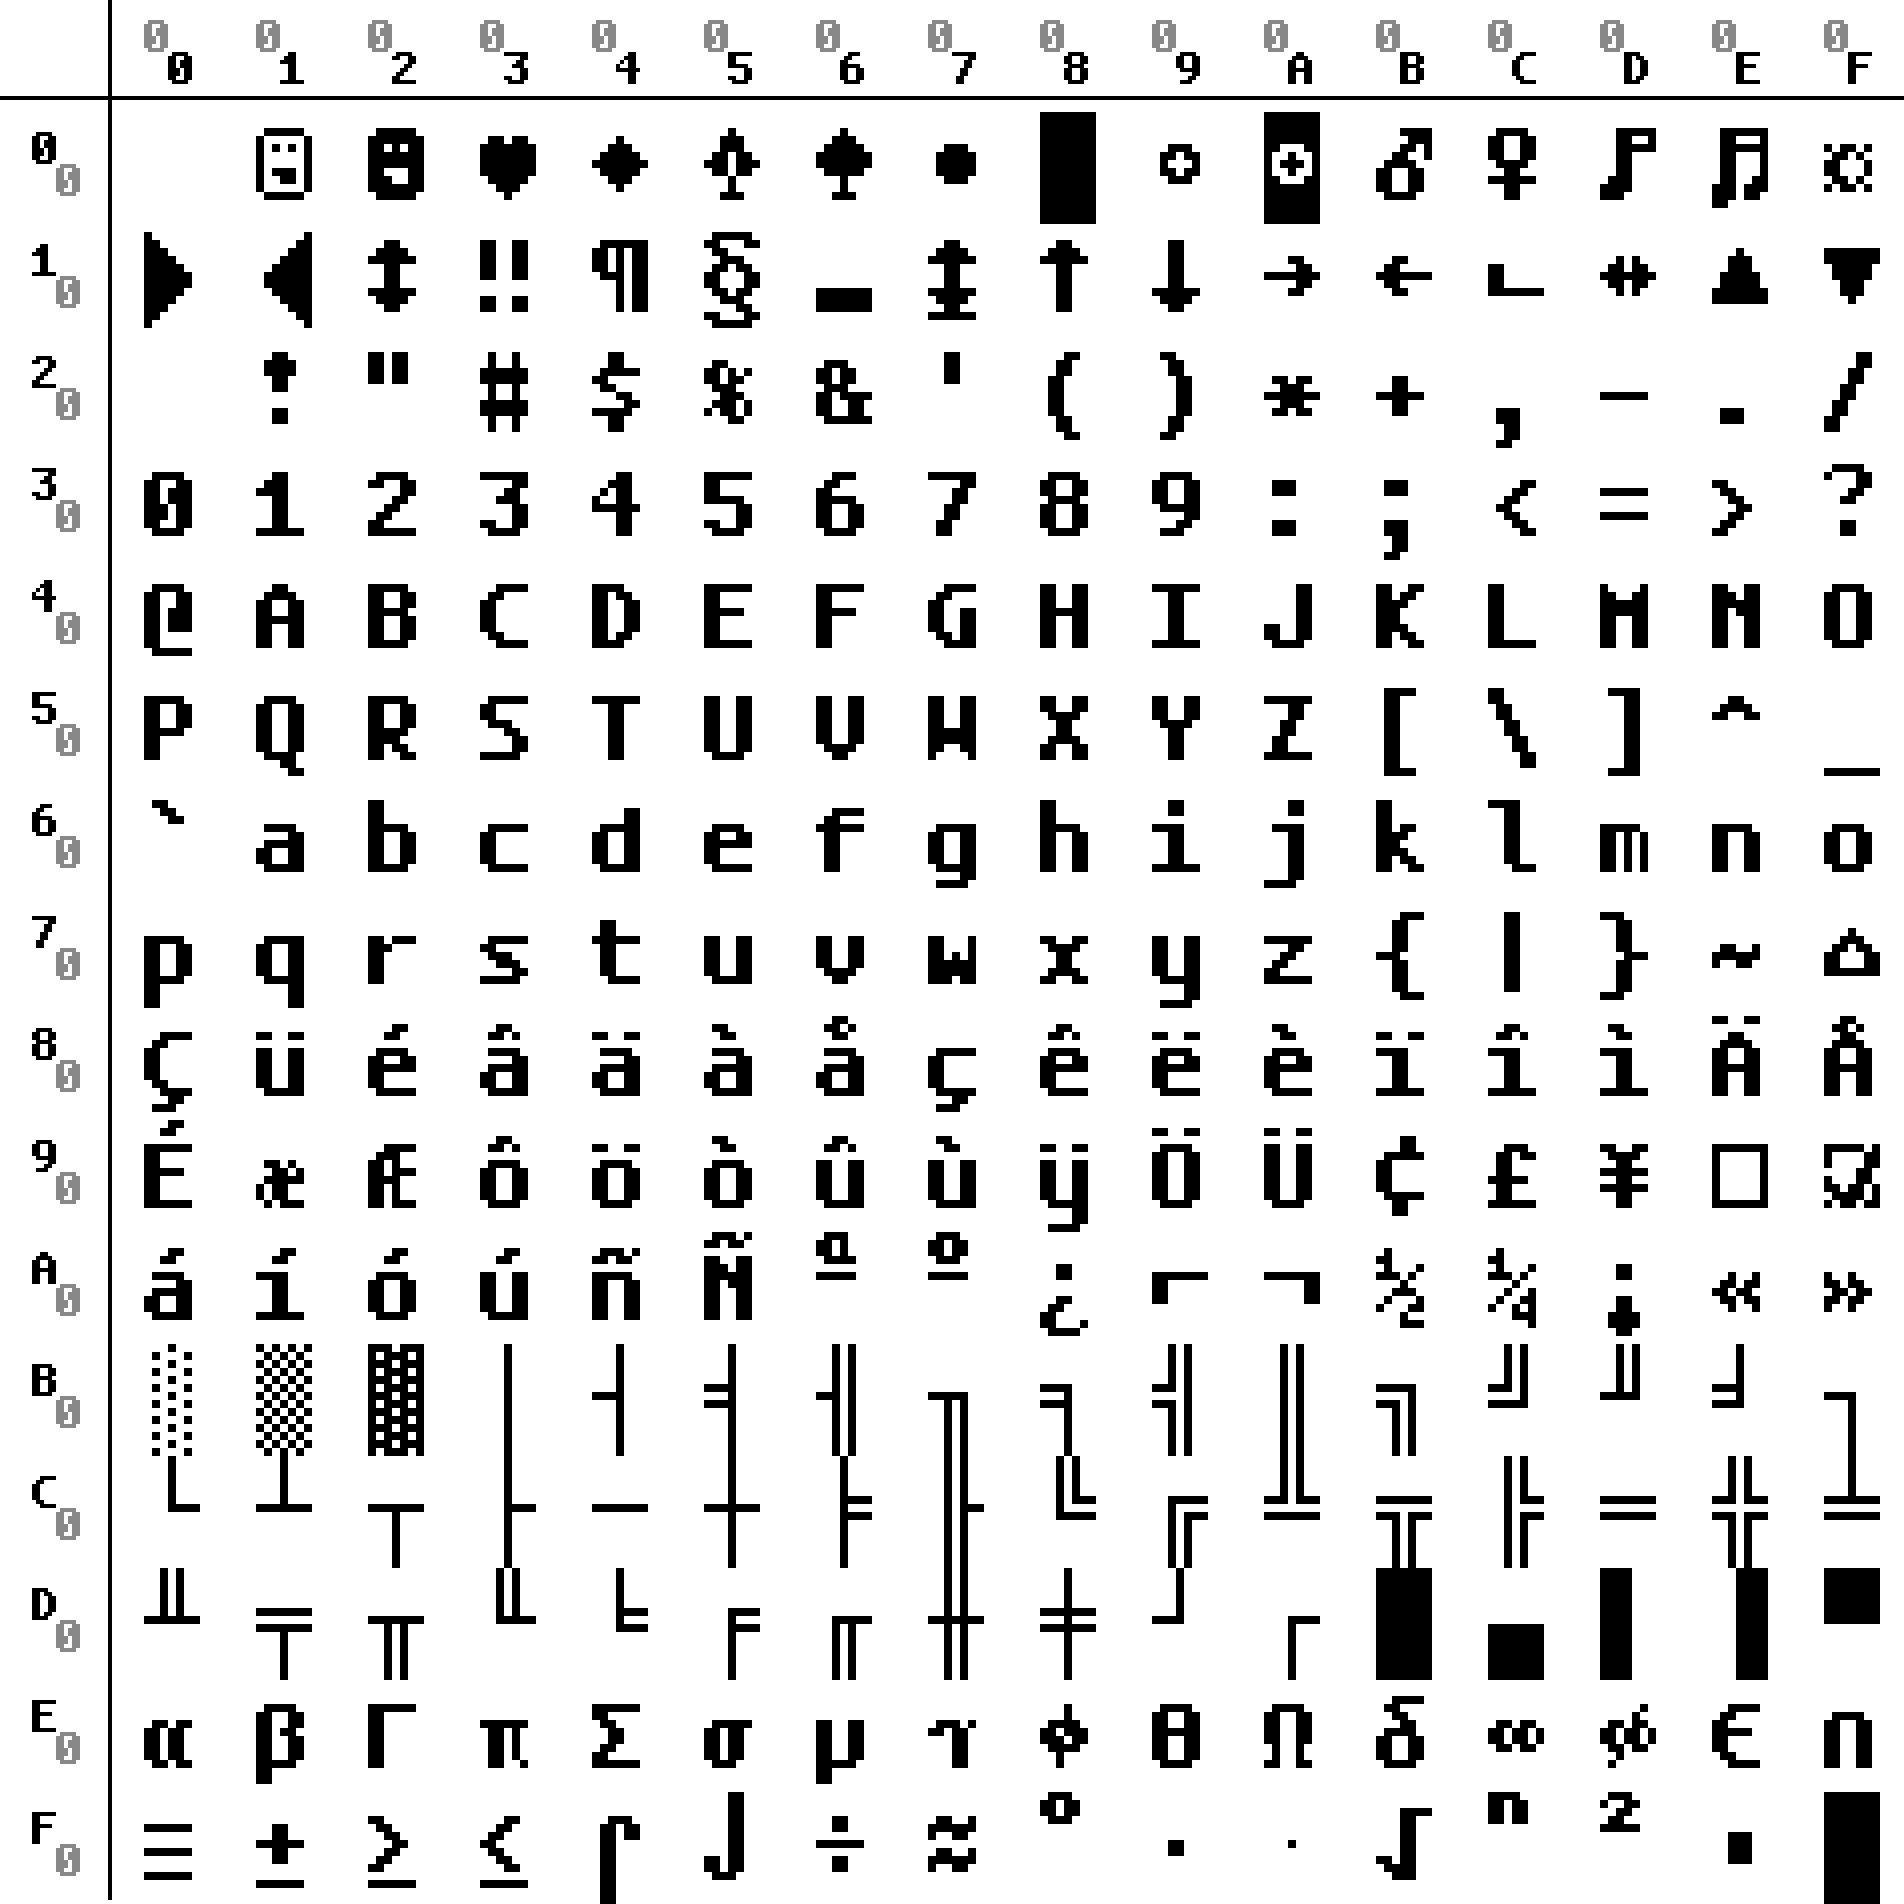
\includegraphics[width=\linewidth]{tsvmcp.png}
\captionof{figure}{\thismachine\ Character Map}
\label{fig:codepage}
}
\newpage

\section{Colour Palette}
\label{colourpalette}

\index{colour palette}By default the reference graphics adapter of the \thismachine\ uses following colour palette:

{\centering
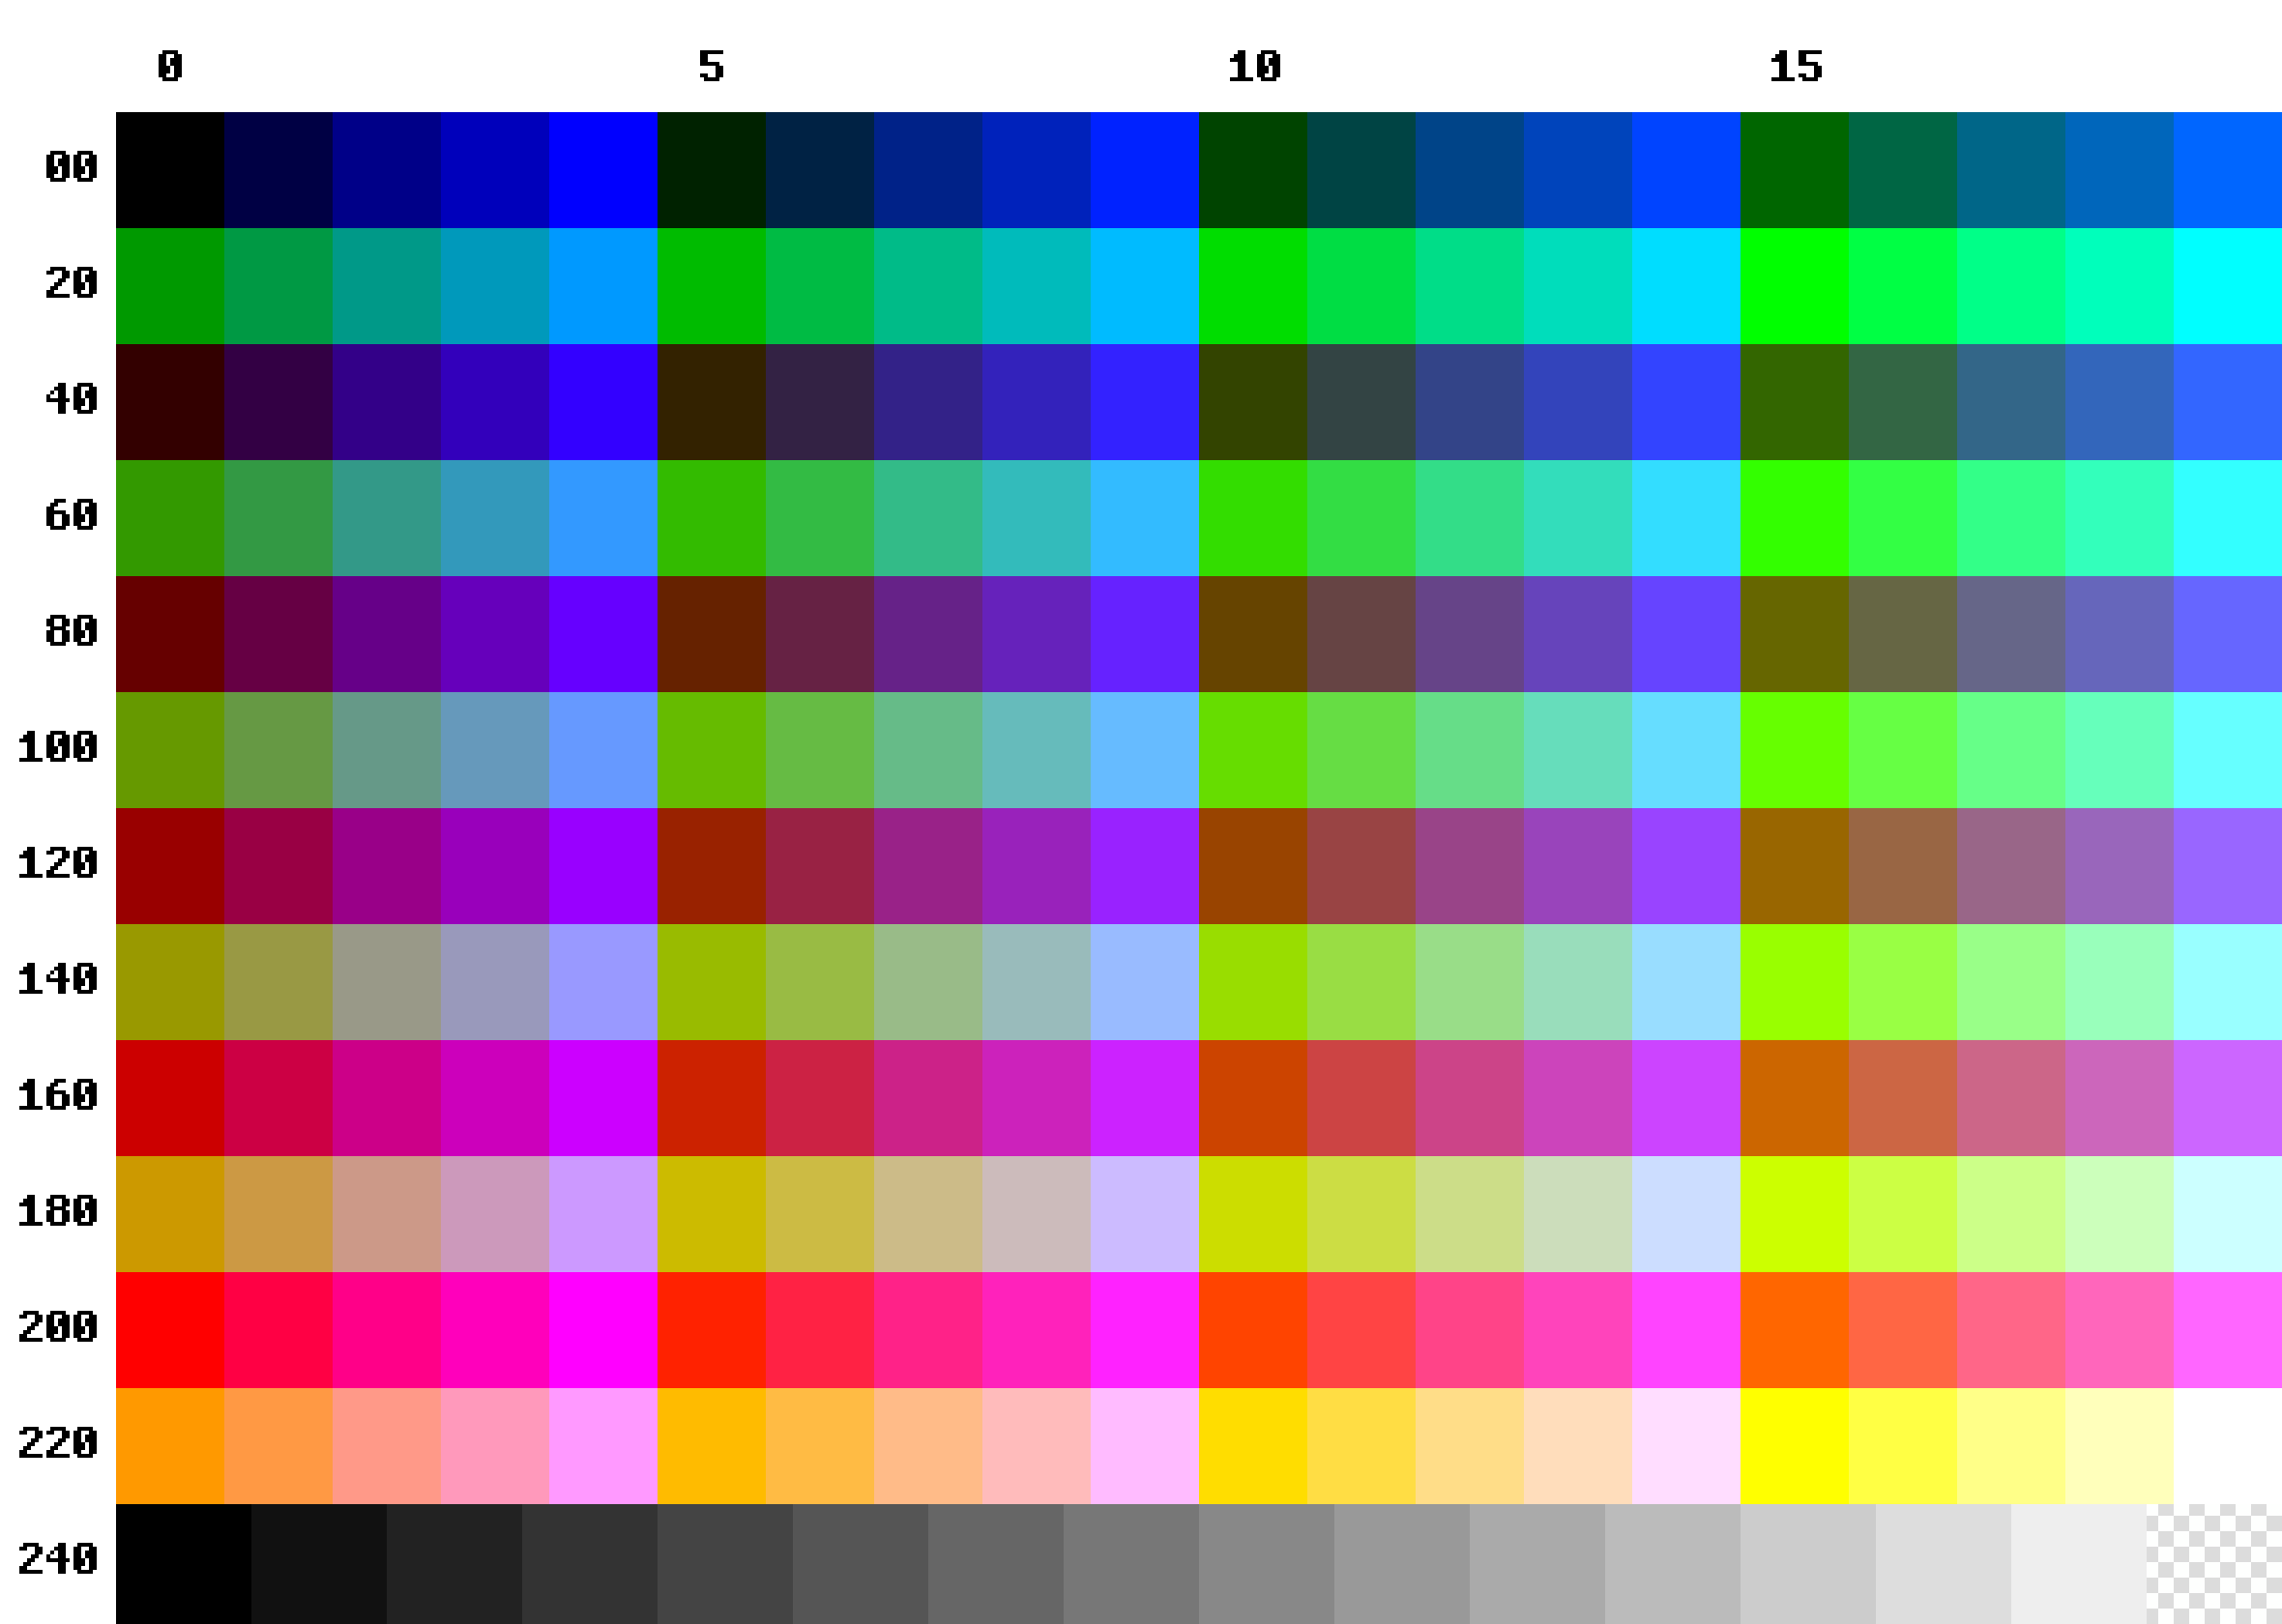
\includegraphics[width=\linewidth]{tsvmpal.png}
\captionof{figure}{\thismachine\ Colour Palette}
\label{fig:codepage}
}

{\centering
\fontsize{7pt}{0pt} % second argument is baselineskip but it's useless in table
\newlength{\extrarowheighttwo}
\setlength{\extrarowheighttwo}{\extrarowheight}
\setlength{\extrarowheight}{-0.2ex}

\begin{longtable}{*{2}{m{\textwidth}}}\hline
\endfirsthead
\endhead

\endfoot
\hline
\endlastfoot
\centering
\begin{tabulary}{\textwidth}{rl}
{\ttfamily 0} & {\ttfamily \#0000} \\
{\ttfamily 1} & {\ttfamily \#0004} \\
{\ttfamily 2} & {\ttfamily \#0008} \\
{\ttfamily 3} & {\ttfamily \#000B} \\
{\ttfamily 4} & {\ttfamily \#000F} \\
{\ttfamily 5} & {\ttfamily \#0020} \\
{\ttfamily 6} & {\ttfamily \#0024} \\
{\ttfamily 7} & {\ttfamily \#0028} \\
{\ttfamily 8} & {\ttfamily \#002B} \\
{\ttfamily 9} & {\ttfamily \#002F} \\
{\ttfamily 10} & {\ttfamily \#0040} \\
{\ttfamily 11} & {\ttfamily \#0044} \\
{\ttfamily 12} & {\ttfamily \#0048} \\
{\ttfamily 13} & {\ttfamily \#004B} \\
{\ttfamily 14} & {\ttfamily \#004F} \\
{\ttfamily 15} & {\ttfamily \#0060} \\
{\ttfamily 16} & {\ttfamily \#0064} \\
{\ttfamily 17} & {\ttfamily \#0068} \\
{\ttfamily 18} & {\ttfamily \#006B} \\
{\ttfamily 19} & {\ttfamily \#006F} \\
{\ttfamily 20} & {\ttfamily \#0090} \\
{\ttfamily 21} & {\ttfamily \#0094} \\
{\ttfamily 22} & {\ttfamily \#0098} \\
{\ttfamily 23} & {\ttfamily \#009B} \\
{\ttfamily 24} & {\ttfamily \#009F} \\
{\ttfamily 25} & {\ttfamily \#00B0} \\
{\ttfamily 26} & {\ttfamily \#00B4} \\
{\ttfamily 27} & {\ttfamily \#00B8} \\
{\ttfamily 28} & {\ttfamily \#00BB} \\
{\ttfamily 29} & {\ttfamily \#00BF} \\
{\ttfamily 30} & {\ttfamily \#00D0} \\
{\ttfamily 31} & {\ttfamily \#00D4} \\
{\ttfamily 32} & {\ttfamily \#00D8} \\
{\ttfamily 33} & {\ttfamily \#00DB} \\
{\ttfamily 34} & {\ttfamily \#00DF} \\
{\ttfamily 35} & {\ttfamily \#00F0} \\
{\ttfamily 36} & {\ttfamily \#00F4} \\
{\ttfamily 37} & {\ttfamily \#00F8} \\
{\ttfamily 38} & {\ttfamily \#00FB} \\
{\ttfamily 39} & {\ttfamily \#00FF} \\
{\ttfamily 40} & {\ttfamily \#0300} \\
{\ttfamily 41} & {\ttfamily \#0304} \\
{\ttfamily 42} & {\ttfamily \#0308} \\
\end{tabulary}
\begin{tabulary}{\textwidth}{|rl}
{\ttfamily 43} & {\ttfamily \#030B} \\
{\ttfamily 44} & {\ttfamily \#030F} \\
{\ttfamily 45} & {\ttfamily \#0320} \\
{\ttfamily 46} & {\ttfamily \#0324} \\
{\ttfamily 47} & {\ttfamily \#0328} \\
{\ttfamily 48} & {\ttfamily \#032B} \\
{\ttfamily 49} & {\ttfamily \#032F} \\
{\ttfamily 50} & {\ttfamily \#0340} \\
{\ttfamily 51} & {\ttfamily \#0344} \\
{\ttfamily 52} & {\ttfamily \#0348} \\
{\ttfamily 53} & {\ttfamily \#034B} \\
{\ttfamily 54} & {\ttfamily \#034F} \\
{\ttfamily 55} & {\ttfamily \#0360} \\
{\ttfamily 56} & {\ttfamily \#0364} \\
{\ttfamily 57} & {\ttfamily \#0368} \\
{\ttfamily 58} & {\ttfamily \#036B} \\
{\ttfamily 59} & {\ttfamily \#036F} \\
{\ttfamily 60} & {\ttfamily \#0390} \\
{\ttfamily 61} & {\ttfamily \#0394} \\
{\ttfamily 62} & {\ttfamily \#0398} \\
{\ttfamily 63} & {\ttfamily \#039B} \\
{\ttfamily 64} & {\ttfamily \#039F} \\
{\ttfamily 65} & {\ttfamily \#03B0} \\
{\ttfamily 66} & {\ttfamily \#03B4} \\
{\ttfamily 67} & {\ttfamily \#03B8} \\
{\ttfamily 68} & {\ttfamily \#03BB} \\
{\ttfamily 69} & {\ttfamily \#03BF} \\
{\ttfamily 70} & {\ttfamily \#03D0} \\
{\ttfamily 71} & {\ttfamily \#03D4} \\
{\ttfamily 72} & {\ttfamily \#03D8} \\
{\ttfamily 73} & {\ttfamily \#03DB} \\
{\ttfamily 74} & {\ttfamily \#03DF} \\
{\ttfamily 75} & {\ttfamily \#03F0} \\
{\ttfamily 76} & {\ttfamily \#03F4} \\
{\ttfamily 77} & {\ttfamily \#03F8} \\
{\ttfamily 78} & {\ttfamily \#03FB} \\
{\ttfamily 79} & {\ttfamily \#03FF} \\
{\ttfamily 80} & {\ttfamily \#0600} \\
{\ttfamily 81} & {\ttfamily \#0604} \\
{\ttfamily 82} & {\ttfamily \#0608} \\
{\ttfamily 83} & {\ttfamily \#060B} \\
{\ttfamily 84} & {\ttfamily \#060F} \\
{\ttfamily 85} & {\ttfamily \#0620} \\
\end{tabulary}
\begin{tabulary}{\textwidth}{|rl}
{\ttfamily 86} & {\ttfamily \#0624} \\
{\ttfamily 87} & {\ttfamily \#0628} \\
{\ttfamily 88} & {\ttfamily \#062B} \\
{\ttfamily 89} & {\ttfamily \#062F} \\
{\ttfamily 90} & {\ttfamily \#0640} \\
{\ttfamily 91} & {\ttfamily \#0644} \\
{\ttfamily 92} & {\ttfamily \#0648} \\
{\ttfamily 93} & {\ttfamily \#064B} \\
{\ttfamily 94} & {\ttfamily \#064F} \\
{\ttfamily 95} & {\ttfamily \#0660} \\
{\ttfamily 96} & {\ttfamily \#0664} \\
{\ttfamily 97} & {\ttfamily \#0668} \\
{\ttfamily 98} & {\ttfamily \#066B} \\
{\ttfamily 99} & {\ttfamily \#066F} \\
{\ttfamily 100} & {\ttfamily \#0690} \\
{\ttfamily 101} & {\ttfamily \#0694} \\
{\ttfamily 102} & {\ttfamily \#0698} \\
{\ttfamily 103} & {\ttfamily \#069B} \\
{\ttfamily 104} & {\ttfamily \#069F} \\
{\ttfamily 105} & {\ttfamily \#06B0} \\
{\ttfamily 106} & {\ttfamily \#06B4} \\
{\ttfamily 107} & {\ttfamily \#06B8} \\
{\ttfamily 108} & {\ttfamily \#06BB} \\
{\ttfamily 109} & {\ttfamily \#06BF} \\
{\ttfamily 110} & {\ttfamily \#06D0} \\
{\ttfamily 111} & {\ttfamily \#06D4} \\
{\ttfamily 112} & {\ttfamily \#06D8} \\
{\ttfamily 113} & {\ttfamily \#06DB} \\
{\ttfamily 114} & {\ttfamily \#06DF} \\
{\ttfamily 115} & {\ttfamily \#06F0} \\
{\ttfamily 116} & {\ttfamily \#06F4} \\
{\ttfamily 117} & {\ttfamily \#06F8} \\
{\ttfamily 118} & {\ttfamily \#06FB} \\
{\ttfamily 119} & {\ttfamily \#06FF} \\
{\ttfamily 120} & {\ttfamily \#0900} \\
{\ttfamily 121} & {\ttfamily \#0904} \\
{\ttfamily 122} & {\ttfamily \#0908} \\
{\ttfamily 123} & {\ttfamily \#090B} \\
{\ttfamily 124} & {\ttfamily \#090F} \\
{\ttfamily 125} & {\ttfamily \#0920} \\
{\ttfamily 126} & {\ttfamily \#0924} \\
{\ttfamily 127} & {\ttfamily \#0928} \\
{\ttfamily 128} & {\ttfamily \#092B} \\
\end{tabulary}
\begin{tabulary}{\textwidth}{|rl}
{\ttfamily 129} & {\ttfamily \#092F} \\
{\ttfamily 130} & {\ttfamily \#0940} \\
{\ttfamily 131} & {\ttfamily \#0944} \\
{\ttfamily 132} & {\ttfamily \#0948} \\
{\ttfamily 133} & {\ttfamily \#094B} \\
{\ttfamily 134} & {\ttfamily \#094F} \\
{\ttfamily 135} & {\ttfamily \#0960} \\
{\ttfamily 136} & {\ttfamily \#0964} \\
{\ttfamily 137} & {\ttfamily \#0968} \\
{\ttfamily 138} & {\ttfamily \#096B} \\
{\ttfamily 139} & {\ttfamily \#096F} \\
{\ttfamily 140} & {\ttfamily \#0990} \\
{\ttfamily 141} & {\ttfamily \#0994} \\
{\ttfamily 142} & {\ttfamily \#0998} \\
{\ttfamily 143} & {\ttfamily \#099B} \\
{\ttfamily 144} & {\ttfamily \#099F} \\
{\ttfamily 145} & {\ttfamily \#09B0} \\
{\ttfamily 146} & {\ttfamily \#09B4} \\
{\ttfamily 147} & {\ttfamily \#09B8} \\
{\ttfamily 148} & {\ttfamily \#09BB} \\
{\ttfamily 149} & {\ttfamily \#09BF} \\
{\ttfamily 150} & {\ttfamily \#09D0} \\
{\ttfamily 151} & {\ttfamily \#09D4} \\
{\ttfamily 152} & {\ttfamily \#09D8} \\
{\ttfamily 153} & {\ttfamily \#09DB} \\
{\ttfamily 154} & {\ttfamily \#09DF} \\
{\ttfamily 155} & {\ttfamily \#09F0} \\
{\ttfamily 156} & {\ttfamily \#09F4} \\
{\ttfamily 157} & {\ttfamily \#09F8} \\
{\ttfamily 158} & {\ttfamily \#09FB} \\
{\ttfamily 159} & {\ttfamily \#09FF} \\
{\ttfamily 160} & {\ttfamily \#0C00} \\
{\ttfamily 161} & {\ttfamily \#0C04} \\
{\ttfamily 162} & {\ttfamily \#0C08} \\
{\ttfamily 163} & {\ttfamily \#0C0B} \\
{\ttfamily 164} & {\ttfamily \#0C0F} \\
{\ttfamily 165} & {\ttfamily \#0C20} \\
{\ttfamily 166} & {\ttfamily \#0C24} \\
{\ttfamily 167} & {\ttfamily \#0C28} \\
{\ttfamily 168} & {\ttfamily \#0C2B} \\
{\ttfamily 169} & {\ttfamily \#0C2F} \\
{\ttfamily 170} & {\ttfamily \#0C40} \\
{\ttfamily 171} & {\ttfamily \#0C44} \\
\end{tabulary}
\begin{tabulary}{\textwidth}{|rl}
{\ttfamily 172} & {\ttfamily \#0C48} \\
{\ttfamily 173} & {\ttfamily \#0C4B} \\
{\ttfamily 174} & {\ttfamily \#0C4F} \\
{\ttfamily 175} & {\ttfamily \#0C60} \\
{\ttfamily 176} & {\ttfamily \#0C64} \\
{\ttfamily 177} & {\ttfamily \#0C68} \\
{\ttfamily 178} & {\ttfamily \#0C6B} \\
{\ttfamily 179} & {\ttfamily \#0C6F} \\
{\ttfamily 180} & {\ttfamily \#0C90} \\
{\ttfamily 181} & {\ttfamily \#0C94} \\
{\ttfamily 182} & {\ttfamily \#0C98} \\
{\ttfamily 183} & {\ttfamily \#0C9B} \\
{\ttfamily 184} & {\ttfamily \#0C9F} \\
{\ttfamily 185} & {\ttfamily \#0CB0} \\
{\ttfamily 186} & {\ttfamily \#0CB4} \\
{\ttfamily 187} & {\ttfamily \#0CB8} \\
{\ttfamily 188} & {\ttfamily \#0CBB} \\
{\ttfamily 189} & {\ttfamily \#0CBF} \\
{\ttfamily 190} & {\ttfamily \#0CD0} \\
{\ttfamily 191} & {\ttfamily \#0CD4} \\
{\ttfamily 192} & {\ttfamily \#0CD8} \\
{\ttfamily 193} & {\ttfamily \#0CDB} \\
{\ttfamily 194} & {\ttfamily \#0CDF} \\
{\ttfamily 195} & {\ttfamily \#0CF0} \\
{\ttfamily 196} & {\ttfamily \#0CF4} \\
{\ttfamily 197} & {\ttfamily \#0CF8} \\
{\ttfamily 198} & {\ttfamily \#0CFB} \\
{\ttfamily 199} & {\ttfamily \#0CFF} \\
{\ttfamily 200} & {\ttfamily \#0F00} \\
{\ttfamily 201} & {\ttfamily \#0F04} \\
{\ttfamily 202} & {\ttfamily \#0F08} \\
{\ttfamily 203} & {\ttfamily \#0F0B} \\
{\ttfamily 204} & {\ttfamily \#0F0F} \\
{\ttfamily 205} & {\ttfamily \#0F20} \\
{\ttfamily 206} & {\ttfamily \#0F24} \\
{\ttfamily 207} & {\ttfamily \#0F28} \\
{\ttfamily 208} & {\ttfamily \#0F2B} \\
{\ttfamily 209} & {\ttfamily \#0F2F} \\
{\ttfamily 210} & {\ttfamily \#0F40} \\
{\ttfamily 211} & {\ttfamily \#0F44} \\
{\ttfamily 212} & {\ttfamily \#0F48} \\
{\ttfamily 213} & {\ttfamily \#0F4B} \\
{\ttfamily 214} & {\ttfamily \#0F4F} \\
\end{tabulary}
\begin{tabulary}{\textwidth}{|rl}
{\ttfamily 215} & {\ttfamily \#0F60} \\
{\ttfamily 216} & {\ttfamily \#0F64} \\
{\ttfamily 217} & {\ttfamily \#0F68} \\
{\ttfamily 218} & {\ttfamily \#0F6B} \\
{\ttfamily 219} & {\ttfamily \#0F6F} \\
{\ttfamily 220} & {\ttfamily \#0F90} \\
{\ttfamily 221} & {\ttfamily \#0F94} \\
{\ttfamily 222} & {\ttfamily \#0F98} \\
{\ttfamily 223} & {\ttfamily \#0F9B} \\
{\ttfamily 224} & {\ttfamily \#0F9F} \\
{\ttfamily 225} & {\ttfamily \#0FB0} \\
{\ttfamily 226} & {\ttfamily \#0FB4} \\
{\ttfamily 227} & {\ttfamily \#0FB8} \\
{\ttfamily 228} & {\ttfamily \#0FBB} \\
{\ttfamily 229} & {\ttfamily \#0FBF} \\
{\ttfamily 230} & {\ttfamily \#0FD0} \\
{\ttfamily 231} & {\ttfamily \#0FD4} \\
{\ttfamily 232} & {\ttfamily \#0FD8} \\
{\ttfamily 233} & {\ttfamily \#0FDB} \\
{\ttfamily 234} & {\ttfamily \#0FDF} \\
{\ttfamily 235} & {\ttfamily \#0FF0} \\
{\ttfamily 236} & {\ttfamily \#0FF4} \\
{\ttfamily 237} & {\ttfamily \#0FF8} \\
{\ttfamily 238} & {\ttfamily \#0FFB} \\
{\ttfamily 239} & {\ttfamily \#0FFF} \\
{\ttfamily 240} & {\ttfamily \#0000} \\
{\ttfamily 241} & {\ttfamily \#0111} \\
{\ttfamily 242} & {\ttfamily \#0222} \\
{\ttfamily 243} & {\ttfamily \#0333} \\
{\ttfamily 244} & {\ttfamily \#0444} \\
{\ttfamily 245} & {\ttfamily \#0555} \\
{\ttfamily 246} & {\ttfamily \#0666} \\
{\ttfamily 247} & {\ttfamily \#0777} \\
{\ttfamily 248} & {\ttfamily \#0888} \\
{\ttfamily 249} & {\ttfamily \#0999} \\
{\ttfamily 250} & {\ttfamily \#0AAA} \\
{\ttfamily 251} & {\ttfamily \#0BBB} \\
{\ttfamily 252} & {\ttfamily \#0CCC} \\
{\ttfamily 253} & {\ttfamily \#0DDD} \\
{\ttfamily 254} & {\ttfamily \#0EEE} \\
{\ttfamily 255} & {\ttfamily \#1000} \\
\, & \, \\
\, & \, \\
\end{tabulary}
\end{longtable}

\captionof{table}{Index--ARGB Table of the Colour Palette}
}

\setlength{\extrarowheight}{\extrarowheighttwo}
